\begin{figure}[t]
    \definecolor{YellowGreen}{RGB}{49,126,53}
    \definecolor{Rhodamine}{RGB}{243,156,146}
    \definecolor{Dandelion}{RGB}{242,193,106}
    \vspace{-0.5\baselineskip}
    \centering
    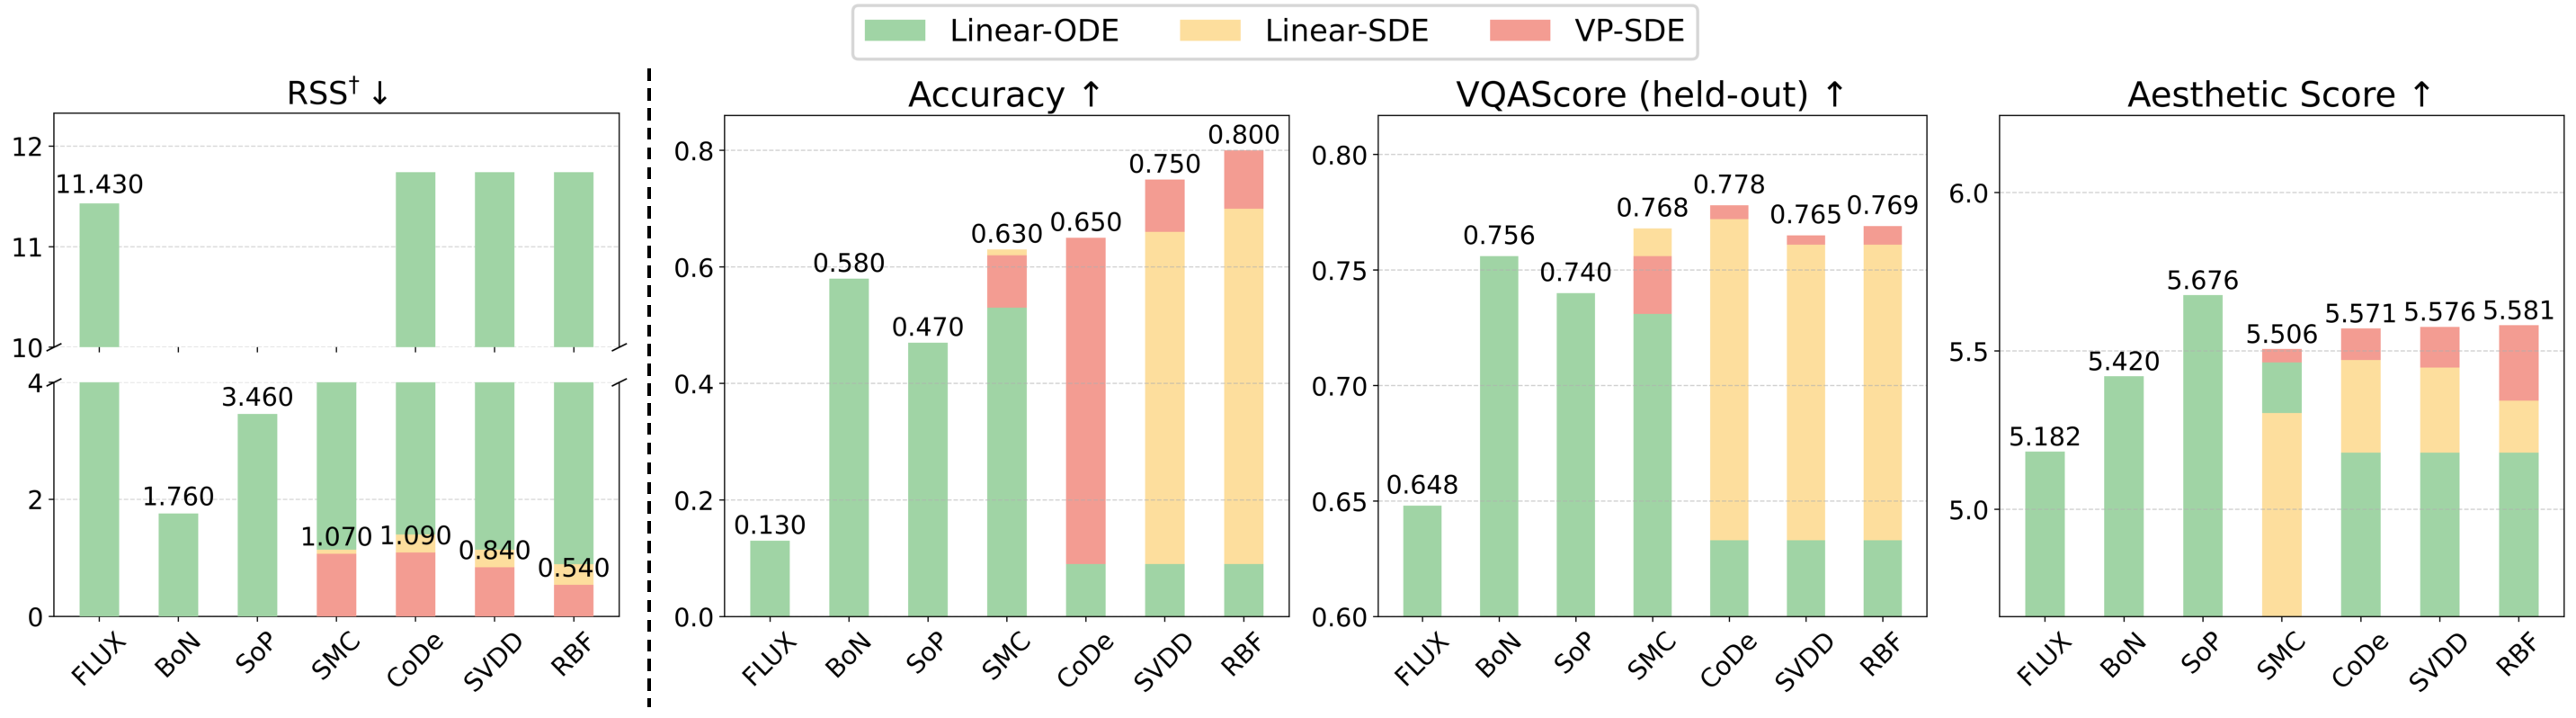
\includegraphics[width=1.0\linewidth]{Tables/quantity_bar_graph/quantity_bar_graph.pdf}
    \caption{\textbf{Quantitative results of quantity-aware image generation.} \textsuperscript{\textdagger} denotes the given reward, RSS~\cite{Liu:2024GroundingDINO}, with the y-axis truncated for better visualization (left). 
    We observe consistent performance improvements by converting {\color{YellowGreen}Linear-ODE} to {\color{Dandelion}{Linear-SDE}}, and {\color{Rhodamine}VP-SDE} for most cases.} 
    \label{fig:counting_main}
    \vspace{-0.75\baselineskip}
\end{figure}


% \begin{table*}[t!]
% \setlength{\tabcolsep}{1.5pt}
% \centering
% \scriptsize
% \renewcommand{\arraystretch}{1.2}
% \caption{\textbf{Quantitative results of quantity-aware image generation.} \textsuperscript{\textdagger} denotes the given reward used in inference-time scaling. The best result in the given and held-out reward is highlighted by \textbf{bold}, and the runner-up is \underline{underlined}. L.O., L.S., and V.S. indicate Linear-ODE, Linear-SDE, and VP-SDE.}
% \vspace{-0.5\baselineskip}
% \label{tab:counting_main}
% \newcolumntype{X}{>{\centering\arraybackslash}m{0.13\linewidth}}
% \newcolumntype{Y}{>{\centering\arraybackslash}m{0.065\linewidth}}
% \newcolumntype{W}{>{\centering\arraybackslash}m{0.045\linewidth}}

% \begin{tabular}{X | Y Y Y | W W W | W W W | W W W | W W W }
% \toprule
% \multirow{2}{*}{Metric} & 
% \multirow{1}{*}{\makecell{FLUX~\cite{BlackForestLabs:2024Flux}}} & 
% \multirow{1}{*}{BoN} & 
% \multirow{1}{*}{\makecell{SoP~\cite{Ma2025:SoP}}} & 
% \multicolumn{3}{c|}{SMC~\cite{Kim:2025DAS}} & 
% \multicolumn{3}{c|}{CoDe~\cite{Singh:2025CoDE}} & 
% \multicolumn{3}{c|}{SVDD~\cite{Li2024:SVDD}} & 
% \multicolumn{3}{c}{{\Oursbf{}} (Ours)} \\
% \cline{2-16}
% & \multicolumn{3}{c|}{L.O.} & L.O. & L.S. & V.S. & L.O. & L.S. & V.S. & L.O. & L.S. & V.S. & L.O. & L.S. & V.S. \\
% \hline
% \makecell{RSS\textsuperscript{\textdagger}\\\cite{Liu:2024GroundingDINO}~$\downarrow$} & 
% 11.430 & 1.760 & 3.460 & 
% 4.870 & 1.140 & 1.070 & 
% 11.740 & 1.400 & 1.090 & 
% 11.740 & 1.140 & \underline{0.840} & 
% 11.740 & 0.890 & \textbf{0.540} \\
% \hline
% \makecell{Accuracy\\\cite{Liu:2024GroundingDINO}~$\uparrow$} & 
% 0.130 & 0.580 & 0.470 & 
% 0.530 & 0.630 & 0.620 & 
% 0.090 & 0.650 & 0.650 & 
% 0.090 & 0.660 & \underline{0.750} & 
% 0.090 & 0.700 & \textbf{0.800} \\
% \hline
% \makecell{VQAScore\\\cite{Lin:2024CLIPFlanT5}~$\uparrow$ (held-out)} & 
% 0.648 & 0.756 & 0.740 & 
% 0.731 & 0.768 & 0.756 & 
% 0.633 & \underline{0.772} & \textbf{0.778} & 
% 0.633 & 0.761 & 0.765 & 
% 0.633 & 0.761 & 0.769 \\
% \hline
% \makecell{Aesthetic\\Score~\cite{Schuhmann:aesthetics}~$\uparrow$} & 
% 5.182 & 5.420 & 5.676 & 
% 5.464 & 5.304 & 5.506 & 
% 5.179 & 5.471 & 5.571 & 
% 5.179 & 5.447 & 5.576 & 
% 5.179 & 5.343 & 5.581 \\
% \bottomrule
% \end{tabular}
% \vspace{-0.5\baselineskip}
% \end{table*}




% previous version
% \begin{table*}[t!]
%     \setlength{\tabcolsep}{1.5pt}
%     \centering
%     \scriptsize
%     \newcommand{\good}[1]{\tiny{\textcolor{blue}{+#1\%}}}
%     \newcommand{\bad}[1]{\tiny{\textcolor{red}{-#1\%}}}
%     \caption{\textbf{Quantitative results of quantity-aware image generation.} \textsuperscript{\textdagger} denotes the given reward used in inference-time scaling. For particle-based sampling methods, the relative improvement in each cell is computed with respect to the Linear-ODE case. The best result in the given and held-out reward is highlighted by \textbf{bold}, and the runner-up is \underline{underlined}. L.O., L.S., and V.S. indicate Linear-ODE, Linear-SDE, and VP-SDE, respectively. \textsuperscript{*} denotes results with $50$ denoising steps.}
%     \vspace{-1.0\baselineskip}
%     \newcolumntype{X}{>{\centering\arraybackslash}m{0.095\linewidth}}
%     \newcolumntype{Y}{>{\centering\arraybackslash}m{0.045\linewidth}}
%     \newcolumntype{Z}{>{\centering\arraybackslash}m{0.05\linewidth}}
%     \newcolumntype{W}{>{\centering\arraybackslash}m{0.035\linewidth}}
%     \begin{tabular}{X | Y Y | Z Z | W W W | W Y Y | W Y Y | W Y Y | W Y Y }
%         \bottomrule
%         \multirow{4}{*}{\makecell{Metric}} & \multicolumn{4}{c|}{\textbf{Diffusion Model}} & \multicolumn{15}{c}{\textbf{Flow Model}} \\
%         \cline{2-20}
%         & \multirow{2}{*}{SD2} & \multirow{2}{*}{$\text{SD2}^{*}$} & \multicolumn{2}{c|}{SVDD~\cite{Li2024:SVDD}} & \multirow{2}{*}{FLUX} & \multirow{2}{*}{BoN} & \multirow{2}{*}{\makecell{SoP\\\cite{Ma2025:SoP}}} & \multicolumn{3}{c|}{\multirow{2}{*}{SMC~\cite{Kim:2025DAS}}} & \multicolumn{3}{c|}{\multirow{2}{*}{CoDe~\cite{Singh:2025CoDE}}} & \multicolumn{3}{c|}{\multirow{2}{*}{SVDD~\cite{Li2024:SVDD}}} & \multicolumn{3}{c}{\multirow{2}{*}{{\Oursbf{}} (Ours)}}\\
%         & & & SD2 & SD2$^{*}$ & & & & & & & & & & & & & & \\
%         % & \multirow{2}{*}{\makecell{SD}} & \multirow{2}{*}{\makecell{$\text{SD}^{*}$}} & \multicolumn{2}{c}{SVDD~\cite{Li2024:SVDD}} & \multirow{2}{*}{FLUX} & \multirow{2}{*}{BoN} & \multirow{2}{*}{SoP~\cite{Ma2025:SoP}} & \multirow{2}{*}{\multicolumn{3}{c|}}{\makecell{SMC \\ \cite{Kim:2025DAS}}} & \multirow{2}{*}{\multicolumn{3}{c|}{\makecell{CoDe \\ \cite{Singh:2025CoDE}}}} & \multirow{2}{*}{\multicolumn{3}{c|}{\makecell{SVDD\\\cite{Li2024:SVDD}}}} & \multirow{2}{*}{\multicolumn{3}{c}}{\makecell{{\Oursbf{}} (Ours)}} \\
        
%         % & \makecell{SD \\ \cite{Rombach:2022LDM}} & \makecell{$\text{SD}^{*}$ \\ \cite{Rombach:2022LDM}} & \makecell{SVDD \\ SD~\cite{Li2024:SVDD}} & \makecell{SVDD \\$\text{SD}^{*}$ \cite{Li2024:SVDD}} & \makecell{FLUX \\ \cite{BlackForestLabs:2024Flux}} & BoN & \makecell{SoP \\ \cite{Ma2025:SoP}} & \multicolumn{3}{c|}{\makecell{SMC \\ \cite{Kim:2025DAS}}} & \multicolumn{3}{c|}{\makecell{CoDe \\ \cite{Singh:2025CoDE}}} & \multicolumn{3}{c|}{\makecell{SVDD \\ \cite{Li2024:SVDD}}} & \multicolumn{3}{c}{\makecell{{\Oursbf{}} (Ours)}} \\
%         \cline{2-20}
%         & \multicolumn{2}{c|}{V.S.} & \multicolumn{2}{c|}{V.S.} & \multicolumn{3}{c|}{L.O.} & L.O. & L.S. & V.S. & L.O. & L.S. & V.S. & L.O. & L.S. & V.S. & L.O. & L.S. & V.S. \\
%         \hline
%         \makecell{RSS\textsuperscript{\textdagger} \cite{Liu:2024GroundingDINO} $\downarrow$} & 22.200 & 18.590 & 5.820 & 5.140 & 11.430 & 1.760 & 3.460 & 4.870 & \makecell{1.140 \\ \good{76.59}} & \makecell{1.070 \\ \good{78.03}} & 11.740 & \makecell{1.400 \\\good{88.07}} & \makecell{1.090 \\\good{90.72}} & 11.740 & \makecell{1.140 \\\good{90.29}} & \makecell{\underline{0.840} \\\good{92.84}} & 11.740 & \makecell{0.890 \\\good{92.42}} & \makecell{\textbf{0.540} \\\good{95.40}} \\
%         \hline
%         \makecell{Accuracy \\ \cite{Liu:2024GroundingDINO} $\uparrow$} & 0.020 & 0.050 & 0.470 & 0.470 & 0.130 & 0.580 & 0.470 & 0.530 & \makecell{0.630 \\\good{18.87}} & \makecell{0.620 \\\good{16.98}} & 0.090 & \makecell{0.650 \\\good{622.22}} & \makecell{0.650 \\\good{622.22}} & 0.090 & \makecell{0.660 \\\good{633.33}} & \makecell{\underline{0.750} \\\good{733.33}} & 0.090 & \makecell{0.700 \\\good{677.78}} & \makecell{\textbf{0.800} \\\good{788.89}} \\
%         \hline
%         \makecell{VQAScore~\cite{Lin:2024CLIPFlanT5} \\ $\uparrow$ (held-out)} & 0.523 & 0.532 & 0.617 & 0.648 & 0.648 & 0.756 & 0.740 & 0.731 & \makecell{0.768 \\\good{5.06}} & \makecell{0.756 \\\good{3.42}} & 0.633 & \makecell{\underline{0.772} \\\good{21.96}} & \makecell{\textbf{0.778} \\\good{22.91}} & 0.633 & \makecell{0.761 \\\good{20.22}} & \makecell{0.765 \\\good{20.85}} & 0.633 & \makecell{0.761 \\\good{20.22}} & \makecell{0.769 \\\good{21.48}} \\
%         \hline
%         \makecell{Aesthetic \\ Score~\cite{Schuhmann:aesthetics} $\uparrow$} & 5.060 & 5.223 & 4.983 & 5.081 & 5.182 & 5.420 & 5.676 & 5.464 & 5.304 & 5.506 & 5.179 & 5.471 & 5.571 & 5.179 & 5.447 & 5.576 & 5.179 & 5.343 & 5.581 \\
%         \toprule
%     \end{tabular}
%     \label{tab:counting_main}
%     \vspace{-0.25\baselineskip}
% \end{table*}


% previous version
% \begin{table*}[t!]
%     \setlength{\tabcolsep}{1.5pt}
%     \centering
%     \scriptsize
%     \newcommand{\good}[1]{\tiny{\textcolor{blue}{+#1\%}}}
%     \newcommand{\bad}[1]{\tiny{\textcolor{red}{-#1\%}}}
%     \caption{\textbf{Quantitative results of quantity-aware image generation.} \textsuperscript{\textdagger} denotes the given reward used in inference-time scaling. For particle-based sampling methods, the relative improvement in each cell is computed with respect to the Linear-ODE case. The best result in the given and held-out reward is highlighted by \textbf{bold}, and the runner-up is \underline{underlined}. L.O., L.S., and V.S. indicate Linear-ODE, Linear-SDE, and VP-SDE, respectively. \textsuperscript{*} denotes results with $50$ denoising steps.}
%     \vspace{-1.0\baselineskip}
%     \newcolumntype{X}{>{\centering\arraybackslash}m{0.095\linewidth}}
%     \newcolumntype{Y}{>{\centering\arraybackslash}m{0.045\linewidth}}
%     \newcolumntype{Z}{>{\centering\arraybackslash}m{0.05\linewidth}}
%     \newcolumntype{W}{>{\centering\arraybackslash}m{0.035\linewidth}}
%     \begin{tabular}{X | Y Y | Z Z | W W W | W Y Y | W Y Y | W Y Y | W Y Y }
%         \bottomrule
%         \multirow{4}{*}{\makecell{Metric}} & \multicolumn{4}{c|}{\textbf{Diffusion Model}} & \multicolumn{15}{c}{\textbf{Flow Model}} \\
%         \cline{2-20}
%         & \multirow{2}{*}{SD2} & \multirow{2}{*}{$\text{SD2}^{*}$} & \multicolumn{2}{c|}{SVDD~\cite{Li2024:SVDD}} & \multirow{2}{*}{FLUX} & \multirow{2}{*}{BoN} & \multirow{2}{*}{\makecell{SoP\\\cite{Ma2025:SoP}}} & \multicolumn{3}{c|}{\multirow{2}{*}{SMC~\cite{Kim:2025DAS}}} & \multicolumn{3}{c|}{\multirow{2}{*}{CoDe~\cite{Singh:2025CoDE}}} & \multicolumn{3}{c|}{\multirow{2}{*}{SVDD~\cite{Li2024:SVDD}}} & \multicolumn{3}{c}{\multirow{2}{*}{{\Oursbf{}} (Ours)}}\\
%         & & & SD2 & SD2$^{*}$ & & & & & & & & & & & & & & \\
%         % & \multirow{2}{*}{\makecell{SD}} & \multirow{2}{*}{\makecell{$\text{SD}^{*}$}} & \multicolumn{2}{c}{SVDD~\cite{Li2024:SVDD}} & \multirow{2}{*}{FLUX} & \multirow{2}{*}{BoN} & \multirow{2}{*}{SoP~\cite{Ma2025:SoP}} & \multirow{2}{*}{\multicolumn{3}{c|}}{\makecell{SMC \\ \cite{Kim:2025DAS}}} & \multirow{2}{*}{\multicolumn{3}{c|}{\makecell{CoDe \\ \cite{Singh:2025CoDE}}}} & \multirow{2}{*}{\multicolumn{3}{c|}{\makecell{SVDD\\\cite{Li2024:SVDD}}}} & \multirow{2}{*}{\multicolumn{3}{c}}{\makecell{{\Oursbf{}} (Ours)}} \\
        
%         % & \makecell{SD \\ \cite{Rombach:2022LDM}} & \makecell{$\text{SD}^{*}$ \\ \cite{Rombach:2022LDM}} & \makecell{SVDD \\ SD~\cite{Li2024:SVDD}} & \makecell{SVDD \\$\text{SD}^{*}$ \cite{Li2024:SVDD}} & \makecell{FLUX \\ \cite{BlackForestLabs:2024Flux}} & BoN & \makecell{SoP \\ \cite{Ma2025:SoP}} & \multicolumn{3}{c|}{\makecell{SMC \\ \cite{Kim:2025DAS}}} & \multicolumn{3}{c|}{\makecell{CoDe \\ \cite{Singh:2025CoDE}}} & \multicolumn{3}{c|}{\makecell{SVDD \\ \cite{Li2024:SVDD}}} & \multicolumn{3}{c}{\makecell{{\Oursbf{}} (Ours)}} \\
%         \cline{2-20}
%         & \multicolumn{2}{c|}{V.S.} & \multicolumn{2}{c|}{V.S.} & \multicolumn{3}{c|}{L.O.} & L.O. & L.S. & V.S. & L.O. & L.S. & V.S. & L.O. & L.S. & V.S. & L.O. & L.S. & V.S. \\
%         \hline
%         \makecell{RSS\textsuperscript{\textdagger} \cite{Liu:2024GroundingDINO} $\downarrow$} & 22.200 & 18.590 & 5.820 & 5.140 & 11.430 & 1.760 & 3.460 & 4.870 & \makecell{1.140 \\ \good{76.59}} & \makecell{1.070 \\ \good{78.03}} & 11.740 & \makecell{1.400 \\\good{88.07}} & \makecell{1.090 \\\good{90.72}} & 11.740 & \makecell{1.140 \\\good{90.29}} & \makecell{\underline{0.840} \\\good{92.84}} & 11.740 & \makecell{0.890 \\\good{92.42}} & \makecell{\textbf{0.540} \\\good{95.40}} \\
%         \hline
%         \makecell{Accuracy \\ \cite{Liu:2024GroundingDINO} $\uparrow$} & 0.020 & 0.050 & 0.470 & 0.470 & 0.130 & 0.580 & 0.470 & 0.530 & \makecell{0.630 \\\good{18.87}} & \makecell{0.620 \\\good{16.98}} & 0.090 & \makecell{0.650 \\\good{622.22}} & \makecell{0.650 \\\good{622.22}} & 0.090 & \makecell{0.660 \\\good{633.33}} & \makecell{\underline{0.750} \\\good{733.33}} & 0.090 & \makecell{0.700 \\\good{677.78}} & \makecell{\textbf{0.800} \\\good{788.89}} \\
%         \hline
%         \makecell{VQAScore~\cite{Lin:2024CLIPFlanT5} \\ $\uparrow$ (held-out)} & 0.523 & 0.532 & 0.617 & 0.648 & 0.648 & 0.756 & 0.740 & 0.731 & \makecell{0.768 \\\good{5.06}} & \makecell{0.756 \\\good{3.42}} & 0.633 & \makecell{\underline{0.772} \\\good{21.96}} & \makecell{\textbf{0.778} \\\good{22.91}} & 0.633 & \makecell{0.761 \\\good{20.22}} & \makecell{0.765 \\\good{20.85}} & 0.633 & \makecell{0.761 \\\good{20.22}} & \makecell{0.769 \\\good{21.48}} \\
%         \hline
%         \makecell{Aesthetic \\ Score~\cite{Schuhmann:aesthetics} $\uparrow$} & 5.060 & 5.223 & 4.983 & 5.081 & 5.182 & 5.420 & 5.676 & 5.464 & 5.304 & 5.506 & 5.179 & 5.471 & 5.571 & 5.179 & 5.447 & 5.576 & 5.179 & 5.343 & 5.581 \\
%         \toprule
%     \end{tabular}
%     \label{tab:counting_main}
%     \vspace{-0.25\baselineskip}
% \end{table*}





% \begin{table}[!t]
%     \setlength{\tabcolsep}{1.5pt}
%     \centering
%     \tiny
%     \newcommand{\good}[1]{\textcolor{red}{(+#1\%)}}
%     \newcommand{\bad}[1]{\textcolor{blue}{(-#1\%)}}
%     % \newcolumntype{X}{>{\columncolor{Yellow}\centering\arraybackslash}m{0.19\linewidth}}
%     \caption{\textbf{Quantitative results of quantity-aware image generation.} \textsuperscript{\textdagger} denotes the given reward used in inference time. For particle-based sampling methods, The relative improvement in each cell is computed with respect to the Linear-ODE. 
%     The best result in the detection score column is highlighted by \textbf{bold}, and the runner-up is \underline{underlined}.}
%     \label{tab:counting_main}
%     \newcolumntype{Z}{>{\centering\arraybackslash}m{0.155\linewidth}}
%     \begin{tabular}{Z Z | Z Z Z | Z }
%         \toprule
%         \multirow{2}{*}{\makecell{Search\\Algorithm}} & \multirow{2}{*}{\makecell{Sampling\\Method}} & 
%         \multicolumn{3}{c|}{Detection Score}
%         & \makecell{Image Quality} \\
%         \cline{3-6}
%         &  & \makecell{\textbf{\textbf{MSE}}\textsuperscript{\textdagger}~\cite{} $\downarrow$} & \makecell{\textbf{Accuracy}\textsuperscript{\textdagger}~\cite{} $\uparrow$} & \makecell{VQAScore~\cite{} $\uparrow$} & \makecell{Aesthetic \\ Score~\cite{} $\uparrow$} \\
%         % \multirow{2}{*}{\makecell{Search\\Algorithm}} & \multirow{2}{*}{\makecell{Sampling\\Method}} & \makecell{\textbf{Reward}} & \makecell{Text Alignment} & \makecell{Image Quality} \\
%         % \cline{3-5}
%         % &  & \makecell{\textbf{VQA Score}~\cite{} $\uparrow$} & \makecell{VQA Score \\ (Inst. BLIP)~\cite{} $\uparrow$} & \makecell{Aesthetic \\ Score~\cite{} $\uparrow$} \\
%         \hline
%         % ------------------------------------------------------------------------------------------
%         \multicolumn{1}{c}{SD~\cite{}} & VP-SDE & 22.200 & 0.020 & 0.523 & 5.060 \\
%         \hline
%         % ------------------------------------------------------------------------------------------
%         \multicolumn{1}{c}{SD~\cite{} x5} & VP-SDE & 18.590 & 0.050 & 0.532 & 5.223 \\
%         \hline
%         % ------------------------------------------------------------------------------------------
%         \multicolumn{1}{c}{SVDD (SD~\cite{})} & VP-SDE & 5.820 & 0.470 & 0.617 & 4.983\\
%         \hline
%         % ------------------------------------------------------------------------------------------
%         \multicolumn{1}{c}{SVDD (SD~\cite{} x5)} & VP-SDE & 5.140 & 0.470 & 0.648 & 5.081 \\
%         \hline
%         % ------------------------------------------------------------------------------------------
%         % ------------------------------------------------------------------------------------------
%         \multicolumn{6}{c}{\textbf{ODE-based Sampling}} \\
%         \hline
%         % ------------------------------------------------------------------------------------------
%         \multicolumn{1}{c}{Flux~\cite{}} & Linear-ODE & 11.430 & 0.130 & 0.648 & 5.182\\
%         \hline
%         % ------------------------------------------------------------------------------------------
%         \multirow{1}{*}{\makecell{BoN~\cite{}}} & Linear-ODE & 1.760 & 0.580 & 0.756 & 5.420 \\
%         \hline
%         % ------------------------------------------------------------------------------------------
%         \multirow{1}{*}{\makecell{SoP~\cite{}}} & Linear-ODE & 3.460 & 0.470 & 0.740 & 5.676 \\
%         % & VP-SDE & 3.080 \good{10.98} & 0.450 \bad{-4.26} & 0.756 \good{2.16} & 5.693 \\
%         \hline
%         % ------------------------------------------------------------------------------------------
%         % ------------------------------------------------------------------------------------------
%         \multicolumn{6}{c}{\textbf{Particle-based Sampling}} \\
%         \hline
%         % ------------------------------------------------------------------------------------------
%         \multirow{3}{*}{DAS} & Linear-ODE & 4.870 & 0.530 & 0.731 & 5.464 \\
%         & Linear-SDE & 1.140 \good{76.59} & 0.630 \good{18.87} & 0.768 \good{5.06} & 5.304 \\
%         & VP-SDE & 1.070 \good{78.03} & 0.620 \good{16.98} & 0.756 \good{3.42} & 5.506 \\
%         \hline
%         % ------------------------------------------------------------------------------------------
%         \multirow{3}{*}{\makecell{CoDe~\cite{}}} & Linear-ODE & 11.740 & 0.090 & 0.633 & 5.179 \\
%         & Linear-SDE & 1.400 \good{88.07} & 0.650 \good{622.22} & \underline{0.772} \good{21.96} & 5.471 \\
%         & VP-SDE & 1.090 \good{90.72} & 0.650 \good{622.22} & \textbf{0.778} \good{22.91} & 5.571 \\
%         \hline
%         % ------------------------------------------------------------------------------------------
%         \multirow{3}{*}{\makecell{SVDD~\cite{}}} & Linear-ODE & 11.740 & 0.090 & 0.633 & 5.179 \\
%         & Linear-SDE & 1.140 \good{90.29} & 0.660 \good{633.33} & 0.761 \good{20.22} & 5.447 \\
%         & VP-SDE & \underline{0.840} \good{92.84} & \underline{0.750} \good{733.33} & 0.765 \good{20.85} & 5.576 \\
%         \hline
%         % ------------------------------------------------------------------------------------------
%         \multirow{3}{*}{\Oursbf{}} & Linear-ODE & 11.740 & 0.090 & 0.633 & 5.179 \\
%         & Linear-SDE & 0.890 \good{92.42} & 0.700 \good{677.78} & 0.761 \good{20.22} & 5.343 \\
%         & VP-SDE & \textbf{0.540} \good{39.33} & \textbf{0.800} \good{14.29} & 0.769 \good{1.05} & 5.581 \\
%         \toprule
%     \end{tabular}
% \end{table}


% \begin{table}[!t]
%     \setlength{\tabcolsep}{2.9pt}
%     \tiny
%     \centering
%     \newcommand{\good}[1]{\textcolor{red}{(+#1\%)}}
%     \newcommand{\bad}[1]{\textcolor{blue}{(-#1\%)}}
%     \caption{\textbf{Quantitative results of quantity-aware image generation.} Superscript\textsuperscript{\textdagger} denotes the known reward. The relative improvement in each cell is computed with respect to the row directly above.}
%     \label{tab:counting_main}
%     % \vspace{-\baselineskip}
%     \newcolumntype{Z}{>{\centering\arraybackslash}m{0.07\textwidth}}
%     \begin{tabular}{Z Z | Z Z | Z Z Z}
%         \toprule
%         \multicolumn{2}{c|}{\tiny{Search Algorithm / Sampler}} & \makecell{MSE\textsuperscript{\textdagger} $\downarrow$} & \tiny{\makecell{Accuracy $\uparrow$}} & \tiny{\makecell{ Image\\Reward $\uparrow$ }} & \tiny{\makecell{Aesthetic \\ Score $\uparrow$}} \\
%         \midrule
%         % ------------------------------------------------------------------------------------------
%         \multicolumn{1}{c}{BoN (SD~\cite{})} & VP-SDE & - & - & - & - \\
%         \midrule
%         % ------------------------------------------------------------------------------------------
%         \multicolumn{1}{c}{BoN (SD~\cite{} x5)} & VP-SDE & - & - & - & - \\
%         \midrule
%         % ------------------------------------------------------------------------------------------
%         \multirow{1}{*}{\makecell{BoN~\cite{}}} & Linear-ODE & - & - & - & - \\
%         \midrule
%         % ------------------------------------------------------------------------------------------
%         \multirow{2}{*}{\makecell{SoP~\cite{}}} & Linear-SDE & - & - & - & - \\
%         & VP-SDE & - & - & - & - \\
%         \midrule
%         % ------------------------------------------------------------------------------------------
%         \multirow{3}{*}{SMC~\cite{}} & Linear-ODE & - & - & - & - \\
%         & Linear-SDE & - & - & - & - \\
%         & VP-SDE & - & - & - & - \\
%         \midrule
%         % ------------------------------------------------------------------------------------------
%         \multirow{3}{*}{\makecell{Block.\\BoK~\cite{}}} & Linear-ODE & - & - & - & - \\
%         & Linear-SDE & - & - & - & - \\
%         & VP-SDE & - & - & - & - \\
%         \midrule
%         % ------------------------------------------------------------------------------------------
%         \multirow{3}{*}{\makecell{BoK~\cite{}}} & Linear-ODE & - & - & - & - \\
%         & Linear-SDE & - & - & - & - \\
%         & VP-SDE & - & - & - & - \\
%         \midrule
%         % ------------------------------------------------------------------------------------------
%         \multirow{2}{*}{\Oursbf{}} & Linear-SDE & - & - & - & - \\
%         & VP-SDE & - & - & - & - \\
%         \bottomrule
%     \end{tabular}
% \end{table}

% ------------------------------------------------------------------------------------------------

% \begin{table}[!t]
%     \setlength{\tabcolsep}{2.9pt}
%     \small
%     \centering
%     \caption{Quantitative results in counting task using 100 prompts in T2I-CompBench~\cite{T2I-CompBench}.}
%     \label{tab:counting_main}
%     % \vspace{-\baselineskip}
%     \newcolumntype{Z}{>{\centering\arraybackslash}m{0.01\textwidth}}
%     \newcolumntype{Y}{>{\centering\arraybackslash}m{0.052\textwidth}}
%     % \newcolumntype{X}{>{\centering\arraybackslash}m{0.066\textwidth}}
%     \newcolumntype{X}{>{\centering\arraybackslash}m{0.086\textwidth}}
%     \begin{tabular}{Z X Y Y Y Y Y Y}
%         \toprule
%         \multicolumn{2}{c}{\textbf{Counting}} & MSE $\downarrow$ & Acc $\uparrow$ & \tiny{UniDet $\uparrow$} & \tiny{\makecell{VQA\\Score}}$\uparrow$ & \tiny{\makecell{Image\\Reward}}$\uparrow$ & \tiny{\makecell{Aesthetic\\Score $\uparrow$}} \\
%         \midrule
%         \multirow{2}{*}{\rotatebox{90}{SD}} & SVDD-10 & 5.820 & 0.470 & 0.505 & 0.617 & -0.006 & 4.983 \\
%         & SVDD-50 & 5.140 & 0.470 & 0.532 & 0.648 & 0.331 & 5.081 \\
%         \midrule
%         \multicolumn{2}{c}{BoN} & 1.760 & 0.580 & 0.600 & 0.756 & 0.895 & 5.420 \\
%         \midrule
%         \multirow{2}{*}{\rotatebox{90}{SoP}} & OT & 3.460 & 0.470 & 0.544 & 0.740 & 0.906 & 5.676 \\
%         & VP & 3.080 & 0.450 & 0.552 & 0.756 & 0.964 & 5.693 \\
%         \midrule
%         \multirow{3}{*}{\rotatebox{90}{SMC}} & OT-ODE & 4.870 & 0.530 & 0.586 & 0.731 & 0.895 & 5.464 \\
%         & OT-SDE & 1.140 & 0.630 & 0.607 & 0.768 & 0.956 & 5.304 \\
%         & VP-SDE & 1.070 & 0.620 & 0.625 & 0.756 & 0.996 & 5.506 \\
%         \midrule
%         \multirow{3}{*}{\rotatebox{90}{CoDe}} & OT-ODE & 11.740 & 0.090 & 0.485 & 0.633 & 0.465 & 5.179 \\
%         & OT-SDE & 1.400 & 0.650 & 0.598 & 0.772 & 0.811 & 5.471 \\
%         & VP-SDE & 1.090 & 0.650 & 0.568 & 0.778 & 0.938 & 5.571 \\
%         \midrule
%         \multirow{3}{*}{\rotatebox{90}{SVDD}} & OT-ODE & 11.740 & 0.090 & 0.485 & 0.633 & 0.465 & 5.179 \\
%         & OT-SDE & 1.140 & 0.660 & 0.603 & 0.761 & 0.812 & 5.447 \\
%         & VP-SDE & 0.840 & 0.750 & 0.574 & 0.765 & 0.927 & 5.576 \\
%         \midrule
%         \multirow{2}{*}{\rotatebox{90}{last}} &  OT-SDE & 0.890 & 0.700 & 0.621 & 0.761 & 0.959 & 5.343 \\
%         & VP-SDE & 0.540 & 0.800 & 0.622 & 0.769 & 0.902 & 5.581 \\
%         \midrule
%         \multirow{2}{*}{\rotatebox{90}{best}} &  OT-SDE & 0.670 & 0.740 & 0.626 & 0.785 & 1.166 & 5.613 \\
%         & VP-SDE & 0.430 & 0.840 & 0.631 & 0.782 & 1.167 & 5.668 \\
%         \bottomrule
%     \end{tabular}
% \end{table}